%!TEX root = ../main.tex
\chapter{Classical Factor Analysis and PCA}

This chapter draws on material from Chapters 11--12 of Murphy's \emph{Machine Learning: A Probabilistic Perspective}, Andrew Ng's lecture notes for CS229 at Stanford, and Jolliffe's \emph{Principal Component Analysis}.

\section{EM Algorithm}


\subsection{The Idea behind the EM Algorithm}
For simplicity, we'll consider an iid setup for now although the EM can be used in situations with dependence. We'll also suppose that the latent variable is continuous. If it's discrete the idea is exactly the same but the integral is replaced by a sum.
	$$\ell(\theta) = \sum_{t=1}^T \log p(\textbf{x}_t;\theta) = \sum_{t=1}^T \log \left(\int p(\textbf{x}_t,	\textbf{z}_t;\theta)\; d \textbf{z} \right)$$
where $\mathbf{x}_t$ is observed and $\mathbf{z}_t$ is unobserved. In many interesting models there is no explicit formula for the MLE in terms of the marginal density $p(\mathbf{x}_t;\theta)$ but there \emph{is} an explicit formula in terms of the \emph{joint} density $p(\mathbf{x}_t,\mathbf{z}_t;\theta)$. This is exactly the setting in which the EM algorithm is useful. Rather than directly maximizing $\ell(\theta)$, the EM algorithm proceeds \emph{iteratively} over the following two steps:
	\begin{description}
		\item[(E-step)] Construct a \emph{lower bound} for $\ell(\theta)$
		\item[(M-step)] Optimize the lower bound over $\theta$
	\end{description}
Roughly speaking, the EM algorithm converts a single complicated optimization problem into a sequence of simple optimization problems. The trick is to ensure that the resulting sequence of estimators converges to the MLE. Jensen's Inequality is the key so I'll briefly remind you of a few importnat facts before proceeding. 

\begin{figure}
	\centering
	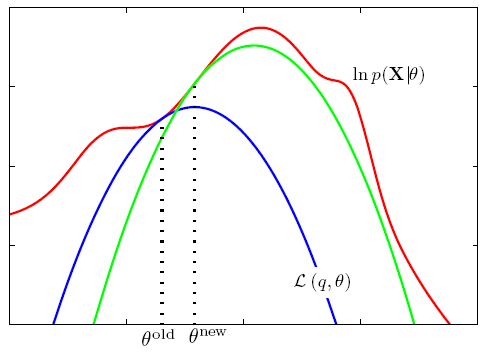
\includegraphics[scale=0.5]{./img/EM_algorithm}
	\caption{Illustration of the EM Algorithm: to maximize the log likelihood, the red curve, we create a sequence of successive approximations, the blue and green curves, and maximize these. This appears as Figure 9.14 in Bishop's (2006) \emph{Pattern Recognitiion and Machine Learning}.}
\end{figure}

\subsection{Jensen's Inequality}
Recall that a function is called \emph{convex} if its Hessian matrix is positive semi-definite and \emph{strictly convex} if its Hessian matrix is positive definite. For functions of a single variable the condition is $f''(x)\geq 0 \quad \forall x\in\mathbb{R}$ for \emph{convex} and $f''(x)> 0 \quad \forall x\in\mathbb{R}$ for \emph{strictly convex}. In statistics, one of the most useful results concerning convex functions is \emph{Jensen's Inequality}
\begin{pro}[Jensen's Inequality]
 	Let $f$ be a convex function and $X$ be a random variable. Then $E[f(X)]\geq f(E[X])$. If $f$ is strictly convex then the inequality is strict unless $P(X = E[X]) = 1$, i.e.\ $X$ is a constant. For the equivalent results for concave functions, simply reverse the inequality.
 \end{pro} 



\subsection{A Lower Bound for the Likelihood}
Let $f_t(\mathbf{z}_t)$ be \emph{some arbitrary} density function over the support of $\mathbf{z}_t$, that is any function satisfying $f_t(\mathbf{z_t})\geq 0$ and
	$$\int f_t(\textbf{z}_t) \;d \textbf{z}_t = 1$$
We have
	\begin{eqnarray*}
		 \ell(\theta) = \sum_{t=1}^T \log p(\textbf{x}_t;\theta) &=& \sum_{t=1}^T \log \left(\int p(\textbf{x}_t,	\textbf{z}_t;\theta)\; d \textbf{z}_t \right)\\
		 	&=&  \sum_{t=1}^T \log \left(\int f_t(\mathbf{z}_t) \left[\frac{p(\textbf{x}_t,	\textbf{z}_t;\theta)}{f_t(\mathbf{z}_t)}\right] d \textbf{z}_t \right)
	\end{eqnarray*}
Now we use Jensen's inequality and the fact that $\log$ is a concave function over its domain to find that
	$$\log \left(\int f_t(\mathbf{z}_t) \left[\frac{p(\textbf{x}_t,	\textbf{z}_t;\theta)}{f_t(\mathbf{z}_t)}\right] d \textbf{z}_t \right) \geq \int f_t(\mathbf{z}_t) \log\left[\frac{p(\textbf{x}_t,\textbf{z}_t;\theta)}{f_t(\mathbf{z}_t)}\right] d \textbf{z}_t $$
What's going on here? Since $f_t$ is a \emph{density} the integral inside the parentheses is \emph{an expectation} of a particular function of the argument of integration $\mathbf{z}_t$. The parameter $\theta$ and the observed vector of realizations $\mathbf{x}_t$ are constants with respect to the integration. Substituting the preceding inequality into the sum, we have established that
	$$\ell(\theta) \geq \sum_{t=1}^T \left(\int f_t(\mathbf{z}_t) \log\left[\frac{p(\textbf{x}_t,\textbf{z}_t;\theta)}{f_t(\mathbf{z}_t)}\right] d \textbf{z}_t \right)$$
for \emph{any} density function $f_t$. This is the \emph{lower bound} for the likelihood that we will use in the E-step. The question is, how should we choose $f_t$? 

The key idea is to turn the \emph{inequality} into an \emph{equality} at a particular value of $\theta$. Intuitively, we want to ensure that, in a given iteration of the algorithm, the  actual likelihood and the lower bound \emph{agree} at the value of $\theta$ that emerged from the \emph{preceding} iteration. In this way, our sequence of approximating functions will ``trace out a path'' along the true likelihood, ultimately ensuring that the EM algorithm will converge to the MLE. Since $\log$ is in fact \emph{strictly} concave, the only way for Jensen's inequality to hold with equality is if 
$$\frac{p(\textbf{x}_t,\textbf{z}_t;\theta)}{f_t(\mathbf{z}_t)} = c$$
for some constant $c$ that \emph{does not depend} on $\mathbf{z}_t$. The question is, how should we choose $f_t$ to achieve this? Rearranging, integrating, and using the fact that $f_t$ is a density,
	\begin{eqnarray*}
		c f_t(\mathbf{z}_t) &=& p(\mathbf{x}_t, \mathbf{z}_t;\theta)\\
		c \int f_t(\mathbf{z}_t) \; d \mathbf{z}_t &=& \int p(\mathbf{x}_t, \mathbf{z}_t;\theta) \; d \mathbf{z}_t\\
		c &=& p(\mathbf{x}_t;\theta) 
	\end{eqnarray*}
Substituting for $c$, solving for $f_t$ and using the definition of a conditional density we have
	$$f_t(\textbf{z}_t)= \frac{p(\textbf{x}_t,\textbf{z}_t;\theta)}{p(\mathbf{x}_t;\theta)} = p(\textbf{z}_t|\textbf{x}_t;\theta)$$
In other words, to make the lower bound hold with equality at a particular value of $\theta$, say $\theta^*$, it suffices to set $f_t$ equal to the \emph{conditional} density of $\mathbf{z}_t$ \emph{given} $\mathbf{x}_t$ \emph{evaluated} at $\theta^*$. Crucially this is a both a probability density and a function of $\mathbf{z}_t$ \emph{only} since we plug in the observed value of $\mathbf{x}_t$.

\subsection{The Algorithm}
In the previous subsection we showed that if we set $f_t(\mathbf{z}_t) = p(\textbf{z}_t|\textbf{x}_t;\theta^*)$ then
	$$\ell(\theta^*) = \sum_{t = 1}^T  \left(\int f_t(\mathbf{z}_t) \log\left[\frac{p(\textbf{x}_t,\textbf{z}_t;\theta^*)}{f_t(\mathbf{z}_t)}\right] d \textbf{z}_t \right)$$
and, more generally for \emph{any} value of $\theta$
	$$\ell(\theta) \geq \sum_{t = 1}^T  \left(\int f_t(\mathbf{z}_t) \log\left[\frac{p(\textbf{x}_t,\textbf{z}_t;\theta)}{f_t(\mathbf{z}_t)}\right] d \textbf{z}_t \right)$$
by Jensen's Inequality. Now we are ready to state the EM algorithm:
\begin{alg}[EM Algorithm]
First select a starting value $\theta^{(1)}$. Then repeat the following two steps repeatedly until convergence
			\begin{description}
			 	\item[(E-step)] For each $t$ set $f_t^{(j-1)}(\mathbf{z}_t) = p(\mathbf{z}_t|\mathbf{x}_t; \theta^{(j-1)})$ where $\theta^{(j-1)}$ is the solution from the M-step of the \emph{preceding} iteration. 
			 	\item[(M-step)] 
			 		$\displaystyle\theta^{(j)} = \underset{\theta \in \Theta}{\arg \max} \sum_{t = 1}^T  \left(\int f_t^{(j-1)}(\mathbf{z}_t) \log\left[\frac{p(\textbf{x}_t,\textbf{z}_t;\theta)}{f_t^{(j-1)}(\mathbf{z}_t)}\right] d \textbf{z}_t \right)$
			 \end{description}
If $j = 2$ then $\theta^{(j-1)}$ is simply the starting value $\theta^{(1)}$.
\end{alg}
Note that in the M-step the argument $\theta$ over which we maximize \emph{only} enters the expression $p(\textbf{x}_t,\textbf{z}_t;\theta)$. The density $f^{(j-1)}(\mathbf{z}_t)$ does \emph{not} depend on $\theta$, it depends on the \emph{constant} $\theta^{(j-1)}$ that solved the M-step of the \emph{previous iteration}. The amazing thing about the EM algorithm is that it is \emph{guaranteed} to converge to a local maximum of the likelihood function: each successive iteration \emph{monotonically} improves the likelihood as we will see below. This fact along the the way we constructed our lower bound to hold with equality at the value of $\theta$ from the \emph{previous} M-step gives us an excellent tool for debugging our code: simply plot
	$$\ell(\theta^{(j)}) = \sum_{t = 1}^T  \left(\int f_t^{(j)}(\mathbf{z}_t) \log\left[\frac{p(\textbf{x}_t,\textbf{z}_t;\theta^{(j)})}{f_t^{(j)}(\mathbf{z}_t)}\right] d \textbf{z}_t \right)$$ 
against $j$. The preceding expression is the \emph{objective function} from the $(j+1)$th M-step evaulated at the \emph{solution} from the $j$th M-step. By construction, this If the is equal to the likelihood evaulated at $\theta^{(j)}$. If the plot is \emph{not} increasing monotonically in $j$, then there must be a bug in your code.

\subsection{Why Does the EM Algorithm Converge?}
Let $\theta^{(j)}$ and $\theta^{(j+1)}$ be two succesive solutions to the M-step of the EM algorithm. We will now show that $\ell(\theta^{(j)}) \leq \theta^{(j+1)}$. In other words, the EM algorithm \emph{monotonically} improves the likelihood in each iteration. Since $\{\theta^{(j)}\}$ is a monotonic sequence, it converges as long as it is bounded (Rudin Theorem 3.14). Since $\ell(\theta^{(1)})$ is a lower bound, if follows that the EM algorithm is \emph{guaranteed} to converge to a local maximum of the likelihood function provided that the likelihood function is bounded above. All that remains is to actually demonstrate that $\ell(\theta^{(j)}) \leq \theta^{(j+1)}$.

By definition, 
	$$\theta^{(j+1)} = \underset{\theta \in \Theta}{\arg \max} \sum_{t = 1}^T  \left(\int f_t^{(j)}(\mathbf{z}_t) \log\left[\frac{p(\textbf{x}_t,\textbf{z}_t;\theta)}{f_t^{(j)}(\mathbf{z}_t)}\right]d \textbf{z}_t \right)$$ 
Now let $\tilde{\theta}$ be some arbitrary value of $\theta$. Since $\theta^{(j+1)}$ is the $\arg \max$, evaluating the objective function at $\tilde{\theta}$ cannot yield a greater value than evaluating it at $\theta^{(j+1)}$. Since this holds for \emph{any} $\tilde{\theta}$ it holds in particular for $\theta^{(j)}$. Hence, 
	\begin{eqnarray*}
		\sum_{t = 1}^T  \left(\int f_t^{(j)}(\mathbf{z}_t) \log\left[\frac{p(\textbf{x}_t,\textbf{z}_t;\theta^{(j+1)})}{f_t^{(j)}(\mathbf{z}_t)}\right] d \textbf{z}_t \right) 
		&\geq& 
		\sum_{t = 1}^T  \left(\int f_t^{(j)}(\mathbf{z}_t) \log\left[\frac{p(\textbf{x}_t,\textbf{z}_t;\theta^{(j)})}{f_t^{(j)}(\mathbf{z}_t)}\right] d \textbf{z}_t \right)\\
		&=& \ell(\theta^{(j)})
	\end{eqnarray*}
since we chose $f^{(j)}_t(\mathbf{z}_t)$ to make Jensen's Inequality strict at $\theta^{(j)}$. Now, recall from above that for \emph{any density} $f_t(\mathbf{z}_t)$ and \emph{any} value of $\theta$,
	$$\ell(\theta) \geq \sum_{t=1}^T \left(\int f_t(\mathbf{z}_t) \log\left[\frac{p(\textbf{x}_t,\textbf{z}_t;\theta)}{f_t(\mathbf{z}_t)}\right] d \textbf{z}_t \right)$$
by Jensen's Inequality. Since this holds in general, it also holds in particular for $\theta = \theta^{(j+1)}$ and $f_t(\mathbf{z}_t)= f_t^{(j)}(\mathbf{z}_t)$. Hence,
	$$\ell(\theta^{(j+1)}) \geq \sum_{t=1}^T \left(\int f_t^{(j)}(\mathbf{z}_t) \log\left[\frac{p(\textbf{x}_t,\textbf{z}_t;\theta^{(j+1)})}{f_t^{(j)}(\mathbf{z}_t)}\right] d \textbf{z}_t \right)$$
Combining the two inequalities gives $\ell(\theta^{(j+1)}) \geq \ell(\theta^{(j)})$ as claimed.


\section{Factor Analysis}

Before we proceed, I'll just remind you of some key facts about normal distributions and we'll need below.

\subsection{Facts about the Multivariate Normal Distribution}
\subsubsection{Linear Combinations}
Suppose that $X \sim N(\mu, \Sigma)$ and $Y = a + BX$ where $a$ is a vector and $B$ a matrix of constants. Then $Y \sim (a + B\mu, B\Sigma B')$.
\subsubsection{Marginals and Conditionals}
Let $X_1$ and $X_2$ be random vectors such that $(X_1' , X_2') \sim N(\mu, \Sigma)$ where
	$$\mu = \left[\begin{array}{c}
		\mu_1 \\ \mu_2
	\end{array}\right], \quad \Sigma = \left[ \begin{array}{cc}
	\Sigma_{11} & \Sigma_{12}\\
	\Sigma_{21} & \Sigma_{22}
	\end{array}\right]
	$$
Then, 
	\begin{eqnarray*}
		X_1 &\sim& N(\mu_1, \Sigma_{11})\\
		X_2 &\sim& N(\mu_2, \Sigma_{22})\\
		X_1|X_2 &\sim& N(\mu_{1|2}, \Sigma_{1|2})
	\end{eqnarray*}
where,
	\begin{eqnarray*}
		\mu_{1|2} &=& \mu_1 + \Sigma_{12}\Sigma_{22}^{-1}(X_2 - \mu_2)\\
		\Sigma_{1|2} &=&\Sigma_{11} - \Sigma_{12} \Sigma_{22}^{-1} \Sigma_{21}
	\end{eqnarray*}

\subsection{The Factor Analysis Model}
Classical Factor Analysis specifies a joint distribution on the observable random $p$-vector $X$ and an unobserved or ``latent'' random $k$-vector $Z$, as follows
	\begin{eqnarray*}
		Z &\sim& N_k(0_k, \mathbf{I}_k)\\
		\epsilon &\sim& N_p(0_p, \Psi)\\
		Z &\perp& \epsilon\\
		X &=& \mu + \Lambda Z + \epsilon
	\end{eqnarray*}
where $\mu$ is a $p\times 1$ vector of parameters, $\Lambda$ is a $p\times k$ matrix of parameters called the \emph{factor loading matrix}, and $\Psi$ is a $p\times p$ \emph{diagonal} matrix of parameters. Factor Analysis can be viewed as a ``low rank parameterization'' of a multivariate normal distribution. The idea is that, while $X$ is a random $p$-vector, its realizations lie \emph{close} to a $k$-dimensional affine subspace: $\Lambda$ maps $Z$ from $\mathbb{R}^k$ to a linear subspace of $\mathbb{R}^p$, $\mu$ shifts this subspace away from the origin, and $\epsilon$ adds axis-aligned Gaussian noise. Hence it makes sense to require that $k$ is strictly less than both $p$, the dimension of $X$, and $T$, the sample size. 

The intution is as follows: Factor Analysis ``forces'' $Z$ to ``explain'' the correlation structure of $X$. This is why $\Psi$ is required to be diagonal. The diagonal elements of $\Psi$ are sometimes called the \emph{idiosyncratic variance terms}, since each corresponds to a \emph{single} component of $X$. This is the key point: \emph{conditional} on the factors $Z$, the elements of $X$ are \emph{independent}. 
\begin{figure}
	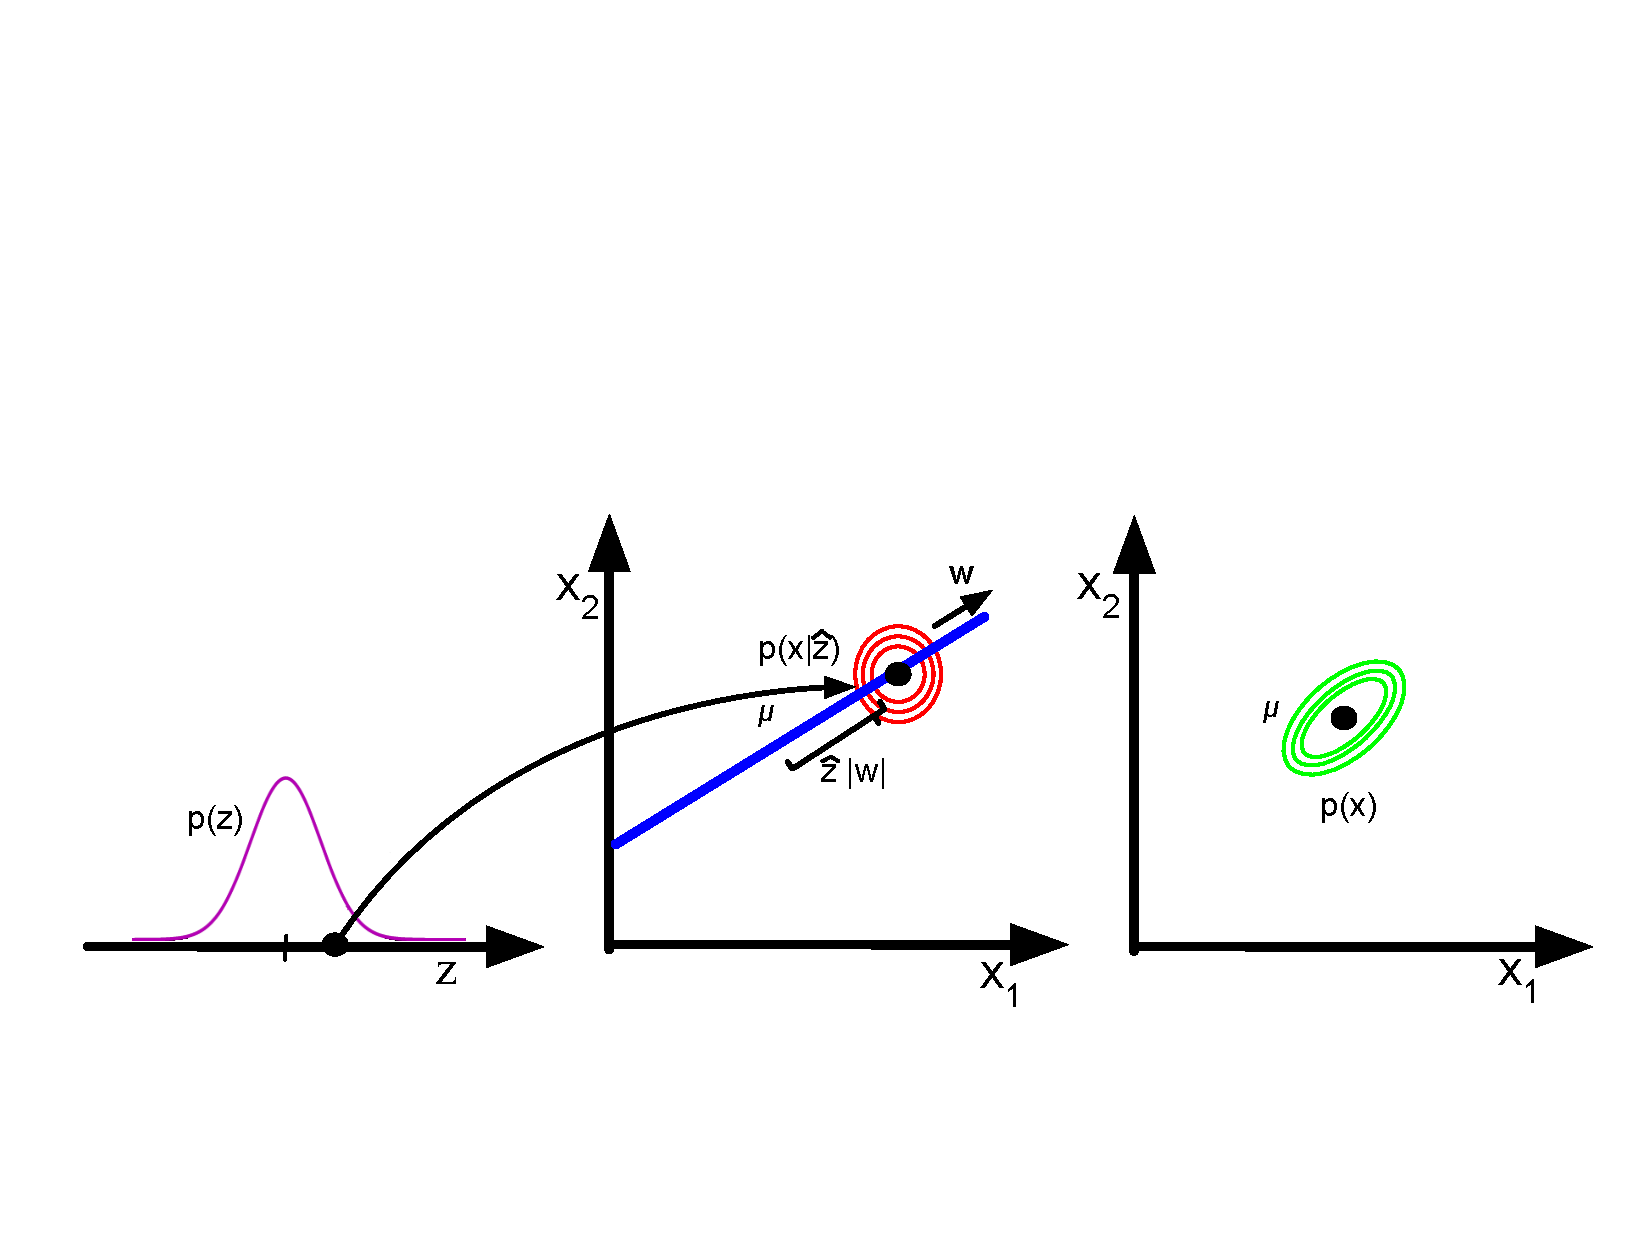
\includegraphics[scale=0.5]{./img/factor_analysis}
	\caption{Illustration of Factor Analysis, although the notation is slightly different from mine. (I need to draw my own version of this.) This appears as figure 12.1 in Murphy (2012).}
\end{figure}

The factor analysis model implies that the joint distribution of $Z$ and $X$ is normal. Specifically,
\begin{eqnarray*}
	\left[\begin{array}{c}
	Z\\ X
	\end{array}\right] &=& 
		\left[\begin{array}{c}
	0_k\\ \mu
	\end{array}\right] + \left[\begin{array}{cc}
		\mathbf{I}_k & 0_{k\times p} \\ \Lambda & I_{p}
	\end{array}\right]\left[\begin{array}{c}
		Z \\ \epsilon
	\end{array} \right]\\
	& = & \left[\begin{array}{c}
	0_k\\ \mu
	\end{array}\right] + \left[\begin{array}{cc}
		\mathbf{I}_k & 0_{k\times p} \\ \Lambda & I_{p}
	\end{array}\right]
	N\left(\left[\begin{array}{c}
		0_k \\ 0_p
	\end{array} \right], \left[\begin{array}{cc}
		\mathbf{I}_k & 0_{k\times p} \\ 0_{p\times k} & \Psi
	\end{array}\right]\right)\\
	&\sim & N\left(\left[\begin{array}{c}
	0_k \\ \mu
	\end{array}\right], \left[\begin{array}{cc}
		I & \Lambda'\\
		\Lambda & \Lambda \Lambda' + \Psi
	\end{array} \right] \right)
\end{eqnarray*}
The algebra for the variance matrix calculation is as follows:
	\begin{eqnarray*}
		V &=& \left[\begin{array}{cc}
		\mathbf{I}_k & 0_{k\times p} \\ \Lambda & I_{p}
	\end{array}\right]
\left[\begin{array}{cc}
		\mathbf{I}_k & 0_{k\times p} \\ 0_{p\times k} & \Psi
	\end{array}\right]
	\left[\begin{array}{cc}
		\mathbf{I}_k & 0_{k\times p} \\ \Lambda & I_{p}
	\end{array}\right]'\\
	&=& \left[ \begin{array}
		{cc} 
		\mathbf{I}_k & 0_{k\times p}\\
		\Lambda & \Psi
	\end{array}\right]\left[\begin{array}{cc}
		\mathbf{I}_k & \Lambda '\\
		0_{p\times k} & I_{p} 
	\end{array}\right]\\
	&=& \left[\begin{array}
		{cc}
		\mathbf{I}_k & \Lambda' \\
		\Lambda & \Lambda \Lambda' + \Psi
	\end{array}\right]
	\end{eqnarray*}


\subsection{The Factor Analysis Model is Not Identified}
Suppose we want to estimated the parameters $\mu, \Lambda, \Psi$ of the factor analysis model. The first natural question is whether this model is even identified. The mean vector $\mu$ doesn't provide any problems for identification since we can always demean $X$ before proceeding. Excluding $\mu$, the factor analysis model has $k(p + 1)$ free parameters: $\Lambda$ is a $p\times k$ matrix and $\Psi$ is a \emph{diagonal} $p\times p$ matrix.


Unfortunately the Factor Analysis is not identified as given above. To see why, suppose that $R$ is an orthogonal matrix, i.e.\ $RR' = R'R = I$. Geometrically, $R$ is a rotation: it leaves the length of any vector $v$ unchanged since
	$$|| Rv || = \sqrt{(Rv)'(Rv)} = \sqrt{v' R'R v} = \sqrt{v'v} = ||v||$$ 
And it leaves the \emph{distance} between any two vectors $v$ and $w$ unchanged since
	\begin{eqnarray*}
		||Rv - Rw|| &=& ||R(v-w)|| = \sqrt{\left[R(v-w) \right]' \left[ R(v-w)\right]}\\
			&=& \sqrt{(v-w)'R'R(v-w)} = \sqrt{(v-w)'(v-w)} = ||v-w||
	\end{eqnarray*}
From the joint distribution for $X$ and $Z$ that we derived above it follows that the marginal distribution of $X$ is $N(\mu, \Lambda \Lambda' + \Psi)$. Thus if we observe realizations $\mathbf{x}_1, \mathbf{x}_2, \hdots, \mathbf{x}_T$ of a sequence of iid random vectors $X_1, X_2, \hdots, X_T$ generated from the Factor Analysis model the log-likelihood is given by
	\begin{eqnarray*}
		\ell(\mu, \Lambda, \Psi) = \log \left[ \prod_{t = 1}^T \frac{\exp \left\{ -\frac{1}{2} \left(\mathbf{x}_t - \mu \right)' \left(\Lambda \Lambda' + \Psi \right)^{-1} \left(\mathbf{x}_t - \mu \right)\right\}}{(2\pi)^{p/2}\left| \Lambda \Lambda' + \Psi \right|^{1/2}} \right] 
	\end{eqnarray*}
Now suppose that we evaluate the log-likelihood at $\widetilde{\Lambda}R$ rather than $\Lambda$. Since $\Lambda$ only enters through the outer product $\Lambda \Lambda'$ the likelihood is \emph{unchanged}: 
	$$\widetilde{\Lambda} \widetilde{\Lambda}' = (\Lambda R)(\Lambda R)' = \Lambda RR' \Lambda' = \Lambda \Lambda'$$
We have shown that the matrix of factor loadings is \emph{only identified up to a rotation}. Another way to think about this is in terms of the latent variable $Z$, Since $X = \mu + \Lambda Z + \epsilon$, post-multiplying $\Lambda$ by $R$ is the same as \emph{pre-multiplying} $Z$ by $R$. As explained above, this constitutes a \emph{rotation} of the vector $Z$. But since $Z$ is a \emph{spherical} normal distribution, rotating it cannot change the likelihood.


If we merely plan to use Factor Analysis for \emph{prediction} this lack of identification is irrelevant: it does not affect the predictive performance of the model in any way. If we ultimately hope to \emph{interpret} the latent factors, however the lack of identification becomes problematic. There are various ways to get a unique solution for the factor loadings $\Lambda$ that involve making various restrictions on the matrix of factor loadings $\Lambda$. The first question is: so how many restrictions do we need?

Since the lack of identication comes from rotational invariance, we need to count the number of free parameters in a $k\times k$ rotation matrix. Start with the first column: it has $k-1$ free parameters since the only constraint is that it have length one. The second column must also have length one, but it has the further restriction that it must be orthogonal to the first column. Hence it has $k - 2$ free parameters. Continuing in this way, we see that there are $(k - 1) + (k - 2) + \hdots + (k - k + 1) = k(k-2)/2$ free parameters in a general $k\times k$ rotation matrix. 

There are a number of possible solutions to the lack of identification:
	\begin{itemize}
		\item \textbf{Constraining the columns of $\Lambda$ to be orthonormal} This is essentially how PCA works, as we'll see below.
		\item \textbf{Constraining $\Lambda$ to be lower triangular} This constraint imposes that the first element of $X$ only depends on the first factor, the second element of $X$ only depends on the first two factors, and so on. In this choice of which variables to list as the first elements of $X$ can make a \emph{big difference}.
		\item \textbf{Imposing Sparsity on $\Lambda$} There are a number of proposals for ``sparse factor analysis,'' including using LASSO and imposing an $\ell_1$ penalty on the factor loadings. Although this might not completely solve the identification problem, setting many of the elements of $\Lambda$ to exactly zero can partially resolve it. 
		\item \textbf{Choosing an Informative Rotation Matrix} If you read old textbooks on multivariate statistics, you'll see a number of suggestions, including something called the ``varimax'' method. Typically, these solutions involve some kind of sparsity condition.
		\item \textbf{Use a Non-Gaussian Distribution for the Factors} The lack of identification in the Factor Analysis Model comes from the rotational invariance of a multivariate normal distribution with an identity covariance matrix. Using a distribution other than the normal can partially eliminate this problem: a Laplace distribution, for example, has diamond-shaped contours. This is the idea behind ``Independent Components Analysis'' (ICA).
	\end{itemize}



\subsection{The Latent Factors}
The unobserved random variables $Z_1, \hdots, Z_T$ that generate $X_1, \hdots, X_T$ under the Factor Analysis Model are called the \emph{latent factors} or the \emph{latent scores}. In some settings the factor scores are given a particular interpretation and we may wish to infer them from the observable data. (Warning: interpreting the factors can be very difficult because of the lack of idenfication of the factor model!) Because this model is Gaussian, we can easily work out the conditional distribution of the latent factors using joint distribution of $(Z',X')'$. Indeed, this is precisely what we'll need to do to implement the EM algorithm, as we'll see below. 


\subsection{Deriving EM for Classical Factor Analysis}
This is a great problem for the EM algorithm since it can be viewed as a case of missing data: if $Z$ were observed, this would just be a standard multivariate regression problem!


\subsubsection{The E-step: Inferring the Latent Factors} In this step we set $f_t^{(j-1)}(\mathbf{z}_t) = p(\mathbf{z}_t|\mathbf{x}_t; \theta^{(j-1)})$ for each $t$ where $\theta^{(j-1)}$ is the value of $\theta$ that solved the optimization problem from the \emph{preceding} M-step or, if $j=2$, the starting value. In the notation of the factor analysis problem we need to calculate:
	$$f_t^{(j-1)}(\mathbf{z}_t) = p(\mathbf{z}_t | \mathbf{x}_t; \mu^{(j-1)}, \Lambda^{(j-1)}, \Psi^{(j-1)})$$
As we showed above,
	\begin{eqnarray*}
		\left[\begin{array}{c}
			Z\\ X
		\end{array}\right] 
		&\sim&  N\left(
		\left[\begin{array}{c}
			0_k \\ \mu
	\end{array}\right], 
		\left[\begin{array}{cc}
			I & \Lambda'\\
			\Lambda & \Lambda \Lambda' + \Psi
		\end{array} \right] \right)
	\end{eqnarray*}
Hence, using the properties of the normal distribution reviewed earlier in this document:
	\begin{eqnarray*}
		Z|X &\sim& N_k(\mu_{Z|X}, \Sigma_{Z|X})\\
		\mu_{Z|X} &=& \Lambda' (\Lambda \Lambda' + \Psi)^{-1}(X - \mu) \\
		\Sigma_{Z|X} &=& \mathbf{I}_k - \Lambda'(\Lambda \Lambda' + \Psi)^{-1}\Lambda
	\end{eqnarray*}
\subsubsection{The M-Step: Optimizing the Lower Bound}
In this step, we solve 
	$$\displaystyle\theta^{(j)} = \underset{\theta \in \Theta}{\arg \max} \sum_{t = 1}^T  \left(\int f_t^{(j-1)}(\mathbf{z}_t) \log\left[\frac{p(\textbf{x}_t,\textbf{z}_t;\theta)}{f_t^{(j-1)}(\mathbf{z}_t)}\right] d \textbf{z}_t \right)$$
Before carrying out the optimization problem, we'll first manipulate the objective function to simplify it and remove constant terms that don't depend on the model parameters. Substituting the notation of the Factor Analysis Model and rearranging, we can write the objective function for the $j$th M-step as follows:
	\begin{eqnarray*}
		Q^{(j)}(\mu, \Lambda, \Psi) &=& \sum_{t=1}^T \int f_t^{(j-1)}(\textbf{z}_t) \log \left[ \frac{p(\textbf{x}_t, \textbf{z}_t;\mu, \Lambda, \Psi)}{f_t^{(j-1)}(\textbf{z}_t)}\right] d \textbf{z}_t\\
			&=&	\sum_{t=1}^T \int f_t^{(j-1)}(\textbf{z}_t) \left[\log p(\textbf{x}_t, \textbf{z}_t;\mu, \Lambda, \Psi) - \log f_t^{(j-1)}(\textbf{z}_t)\right] d \textbf{z}_t\\
		&=&\sum_{t=1}^T \int f_t^{(j-1)}(\textbf{z}_t) \log p(\textbf{x}_t, \textbf{z}_t;\mu, \Lambda, \Psi)\;d \textbf{z}_t -\sum_{t=1}^T  \int f_t^{(j-1)}(\textbf{z}_t) \log f_t^{(j-1)}(\textbf{z}_t) \;d \textbf{z}_t\\
		&=&\sum_{t=1}^T \int f_t^{(j-1)}(\textbf{z}_t) \log p(\textbf{x}_t, \textbf{z}_t;\mu, \Lambda, \Psi)\;d \textbf{z}_t  + C\\
		&=& \sum_{t=1}^T \int f_t^{(j-1)}(\textbf{z}_t) \log p(\textbf{x}_t, \textbf{z}_t;\mu, \Lambda, \Psi)\;d \textbf{z}_t -\sum_{t=1}^T  \int f_t^{(j-1)}(\textbf{z}_t) \log f_t^{(j-1)}(\textbf{z}_t) \;d \textbf{z}_t\\
		&=&\sum_{t=1}^T \int f_t^{(j-1)}(\textbf{z}_t) \log\left[ p(\textbf{x}_t| \textbf{z}_t;\mu, \Lambda, \Psi)p(\textbf{z}_t) \right]d \textbf{z}_t  + C\\
		&=&\sum_{t=1}^T \int f_t^{(j-1)}(\textbf{z}_t) \log p(\textbf{x}_t| \textbf{z}_t;\mu, \Lambda, \Psi)\;d \textbf{z}_t + \sum_{t=1}^T \int f_t^{(j-1)}(\textbf{z}_t)\log p(\textbf{z}_t)\; d \mathbf{z}_t + C\\
		&=& \sum_{t=1}^T \int f_t^{(j-1)}(\textbf{z}_t) \log p(\textbf{x}_t| \textbf{z}_t;\mu, \Lambda, \Psi)\;d \textbf{z}_t + C
	\end{eqnarray*} 
where $C$ denotes an arbitrary constant and we have used the fact that $p(\mathbf{z}_t)$ \emph{does not depend} on any of the model parameters since $Z \sim N_k(0, I)$. 

Writing the joint distribution with $X$ as the first block rather than $Z$, we have
	\begin{eqnarray*}
		\left[\begin{array}{c}
			X\\ Z
		\end{array}\right] 
		&\sim&  N\left(
		\left[\begin{array}{c}
			 \mu \\ 0_k 
	\end{array}\right], 
		\left[\begin{array}{cc}
			 \Lambda \Lambda' + \Psi & \Lambda\\
			 \Lambda' & I
		\end{array} \right] \right)
	\end{eqnarray*}
Hence, using the properties of normal distributions
	\begin{eqnarray*}
		X | Z &\sim& N_p(\mu_{X|Z}, \Sigma_{X|Z})\\
		\mu_{X|Z} &=& \mu + \Lambda Z \\
		\Sigma_{X|Z} &=& \Psi
	\end{eqnarray*}
so 
	$$p(\textbf{x}_t| \textbf{z}_t;\mu, \Lambda, \Psi) = \frac{\exp \left\{-\frac{1}{2}(\mathbf{x}_t - \mu -  \Lambda \textbf{z}_t)' \Psi^{-1} (\mathbf{x}_t - \mu -  \Lambda \textbf{z}_t) \right\}}{{(2\pi)^{p/2}\left|\Psi \right|^{1/2}}}$$
and hence
	$$\log p(\textbf{x}_t| \textbf{z}_t;\mu, \Lambda, \Psi) = -\frac{1}{2}\left[  \log |\Psi| + p \log(2\pi) +(\mathbf{x}_t - \mu -  \Lambda \textbf{z}_t)' \Psi^{-1} (\mathbf{x}_t - \mu -  \Lambda \textbf{z}_t)\right] $$


\paragraph{Updating $\Lambda$:}
Differentiating, 
	\begin{eqnarray*}
		\nabla_\Lambda \log p(\textbf{x}_t| \textbf{z}_t;\mu, \Lambda, \Psi) &=&  \nabla_\Lambda \left[ \frac{1}{2}(\mathbf{x}_t - \mu)' \Psi^{-1} \Lambda \mathbf{z}_t + \frac{1}{2} \mathbf{z}_t' \Lambda'\Psi^{-1} (\mathbf{x}_t - \mu)- \frac{1}{2} \mathbf{z}_t' \Lambda' \Psi^{-1} \Lambda \mathbf{z}_t \right] \\
		&=& \nabla_\Lambda \left[  \mathbf{z}_t' \Lambda'\Psi^{-1} (\mathbf{x}_t - \mu)- \frac{1}{2} \mathbf{z}_t' \Lambda' \Psi^{-1} \Lambda \mathbf{z}_t \right]\\
		&=& \nabla_\Lambda \left[  \mbox{tr}\left\{\mathbf{z}_t' \Lambda'\Psi^{-1} (\mathbf{x}_t - \mu)\right\}- \frac{1}{2} \mbox{tr}\left\{ \mathbf{z}_t' \Lambda' \Psi^{-1} \Lambda \mathbf{z}_t \right\}\right]\\
		&=& \nabla_\Lambda \mbox{tr}\left\{ \Lambda'\Psi^{-1} (\mathbf{x}_t - \mu)\mathbf{z}_t'\right\}- \frac{1}{2} \nabla_\Lambda \mbox{tr}\left\{  \Lambda' \Psi^{-1} \Lambda \mathbf{z}_t \mathbf{z}_t'\right\}
	\end{eqnarray*}
where we have used the fact that each term is a scalar, and thus equals its trace, and $\mbox{tr}(AB) = \mbox{tr}(BA)$ with $\mathbf{z}_t$ playing the role of $A$.

It remains to calculate two matrix derivatives. For the first term we need to calculate $\nabla_X \mbox{tr}(X'A)$ where $\Lambda$ plays the role of $X$ and $\Psi^{-1}(\mathbf{x}_t - \mu)\mathbf{z}_t'$ plays the role of $A$. It turns out that\footnote{See, inter alia, Peterson \& Pederson (2012) \emph{The Matrix Cookbook}, Section 2.5.1 or the Wikipedia article on Matrix Calculus.} 
	$$\nabla_X \mbox{tr}(X'A)  = A$$
For the second term we need to calculate $\nabla_A \mbox{tr}(X'BXC)$ where $\Lambda$ plays the role of $X$, $\Psi^{-1}$ plays the role of $B$, and $\mathbf{z}_t \mathbf{z}_t'$ plays the role of $C$. It turns out that\footnote{Ibid.}
	$$\mbox{tr}(X'BXC) = BXC + BXC'$$
Finally, we have,
	\begin{eqnarray*}
		\nabla_\Lambda \log p(\textbf{x}_t| \textbf{z}_t;\mu, \Lambda, \Psi) &=& \Psi^{-1} (\textbf{x}_t - \mu)\textbf{z}_t' - \frac{1}{2} \left(\Psi^{-1}\Lambda \textbf{z}_t \textbf{z}_t' +  \Psi^{-1}\Lambda \textbf{z}_t \textbf{z}_t'\right)\\
		&=&\Psi^{-1} (\textbf{x}_t - \mu)\textbf{z}_t' - \Psi^{-1}\Lambda \textbf{z}_t \textbf{z}_t' 
	\end{eqnarray*}
Thus, the first order condition for $\Lambda$ is
$$\sum_{t = 1}^T \int f_t^{(j-1)}(\mathbf{z}_t) \left[ \Psi^{-1} (\textbf{x}_t - \mu)\textbf{z}_t' - \Psi^{-1}\Lambda \textbf{z}_t \textbf{z}_t' \right] d \mathbf{z}_t = 0$$
Rearranging,
	\begin{eqnarray*}
		 \Psi^{-1} \sum_{t = 1}^T  (\textbf{x}_t - \mu)\int f_t^{(j-1)}(\mathbf{z}_t) \; \textbf{z}_t' \; d \mathbf{z}_t &=&  \Psi^{-1} \Lambda \sum_{t=1}^T \int f_t^{(j-1)}(\mathbf{z}_t)\; \textbf{z}_t \textbf{z}_t' \; d \mathbf{z}_t\\
		  \sum_{t = 1}^T  (\textbf{x}_t - \mu)\int f_t^{(j-1)}(\mathbf{z}_t) \; \textbf{z}_t' \; d \mathbf{z}_t &=& \Lambda \left(\sum_{t=1}^T \int f_t^{(j-1)}(\mathbf{z}_t)\; \textbf{z}_t \textbf{z}_t' \; d \mathbf{z}_t\right)
	\end{eqnarray*}
Solving for $\Lambda$ and substituting the result of the E-step,
	\begin{eqnarray*}
		\Lambda^{(j)} &=& \left(\sum_{t = 1}^T  (\textbf{x}_t - \mu)\int f_t^{(j-1)}(\mathbf{z}_t) \; \textbf{z}_t' \; d \mathbf{z}_t\right) \left(\sum_{t=1}^T \int f_t^{(j-1)}(\mathbf{z}_t)\; \textbf{z}_t \textbf{z}_t' \; d \mathbf{z}_t\right)^{-1}\\
			&=&\left(\sum_{t = 1}^T  (\textbf{x}_t - \mu)\int \mathcal{N}\left(\mathbf{z}_t|\mu^{(j-1)}_{\mathbf{z}_t|\mathbf{x}_t}, \Sigma^{(j-1)}_{\mathbf{z}_t|\mathbf{x}_t}\right) \; \textbf{z}_t' \; d \mathbf{z}_t\right) \left(\sum_{t=1}^T \int \mathcal{N}\left(\mathbf{z}_t|\mu^{(j-1)}_{\mathbf{z}_t|\mathbf{x}_t}, \Sigma^{(j-1)}_{\mathbf{z}_t|\mathbf{x}_t}\right)\; \textbf{z}_t \textbf{z}_t' \; d \mathbf{z}_t\right)^{-1}\\
			&=& \left[\sum_{t=1}^T (\mathbf{x}_t - \mu)\left(\mu^{(j-1)}_{\mathbf{z}_t|\mathbf{x}_t} \right)'\right]\left[\sum_{t=1}^T \left\{ \left(\mu^{(j-1)}_{\mathbf{z}_t|\mathbf{x}_t} \right)\left(\mu^{(j-1)}_{\mathbf{z}_t|\mathbf{x}_t} \right)' + \left(\Sigma^{(j-1)}_{\mathbf{z}_t|\mathbf{x}_t} \right) \right\}  \right]^{-1}\\
	\end{eqnarray*}
where $\mathcal{N}(\mathbf{z}|\mu, \Sigma)$ denotes a multivariate normal density with argument $\mathbf{z}$, mean $\mu$ and variance matrix $\Sigma$ and
	\begin{eqnarray*}
		\mu^{(j-1)}_{\mathbf{z}_t|\mathbf{x}_t} &=& \left(\Lambda^{(j-1)}\right)' \left[\Lambda^{(j-1)} \left(\Lambda^{(j-1)}\right)' + \Psi^{(j-1)}\right]^{-1} \left(\mathbf{x}_t - \mu^{(j-1)}\right) \\
		\Sigma^{(j-1)}_{\mathbf{z}_t|\mathbf{x}_t}  &=& \mathbf{I} - \left(\Lambda^{(j-1)}\right)' \left[\Lambda^{(j-1)} \left(\Lambda^{(j-1)}\right)' + \Psi^{(j-1)}\right]^{-1}\Lambda^{(j-1)}
	\end{eqnarray*}
Notice that the M-step update for $\Lambda$ looks what would be the multivariate OLS estimator if $Z$ were observed: $\Lambda' = (Z'Z)^{-1}Z'X$. Since we don't observe $Z$ we substitute its conditional mean given $X$. The only twist is the conditional variance term in the term that serves as the analogue of $(Z'Z)^{-1}$. This accounts for the uncertainty in our estimate of $Z$ based on observing $X$.

\paragraph{Updating $\mu$:} Differentiating and rearranging, 
 \begin{eqnarray*}
 	\nabla_\mu \log p(\mathbf{x}_t|\mathbf{z}_t;\mu, \Lambda, \Psi) &=& -\frac{1}{2} \nabla_\mu \left( -\mu' \Psi^{-1} \mathbf{x}_t + \mu' \Psi^{-1}\mu + \mu' \Psi^{-1} \Lambda \mathbf{z}_t - \mathbf{x}_t' \Psi^{-1} \mu +  \mathbf{z}_t'\Lambda' \Psi^{-1} \mu  \right)\\
 		&=& \nabla_\mu \left(\mathbf{x}_t' \Psi^{-1} \mu - \mathbf{z}_t' \Lambda' \Psi^{-1}\mu - \frac{1}{2} \mu' \Psi^{-1} \mu \right)\\
 		&=& \left(\mathbf{x}_t' \Psi^{-1}\right)' - \left(\mathbf{z}_t'\Lambda'\Psi^{-1}\right)' - \Psi^{-1}\mu\\
 		&=& \Psi^{-1}\left(\mathbf{x}_t  - \Lambda\mathbf{z}_t - \mu\right)
 \end{eqnarray*}
where we have used the results $\nabla_{\mathbf{x}}\mathbf{a}' \mathbf{x} = \mathbf{a}$ and$\nabla_{\mathbf{x}}\mathbf{x}'A \mathbf{x} = (A + A')\mathbf{x}$ along with the fact that $\Psi^{-1}$ is symmetric.\footnote{See, inter alia, Peterson \& Pederson (2012) \emph{The Matrix Cookbook}, Section 2.4.1--2 or the Wikipedia article on Matrix Calculus.} Hence the first-order condition for $\mu$ is
$$\sum_{t = 1}^T \int f_t^{(j-1)}(\mathbf{z}_t) \left[\Psi^{-1}\left(\mathbf{x}_t  - \Lambda\mathbf{z}_t - \mu\right) \right] d \mathbf{z}_t = 0$$
Left-multiplying both sides by $\Psi$, using the fact that $f_t^{(j-1)}(\mathbf{z}_t)$ is a density, and substituting the E-step gives
	\begin{eqnarray*}
		\sum_{t = 1}^T \left( \mathbf{x}_t - \Lambda \int f_t^{(j-1)}(\mathbf{z}_t) \; \mathbf{z}_t \; d \mathbf{z}_t - \mu\right)   &=& 0\\
 T\bar{\mathbf{x}} - \Lambda \sum_{t = 1}^T \int f_t^{(j-1)}(\mathbf{z}_t) \; \mathbf{z}_t \; d\mathbf{z}_t &=& T \mu \\
 	\bar{\mathbf{x}}  - \Lambda \left( \frac{1}{T} \sum_{t=1}^T \mu^{(j-1)}_{\mathbf{z}_t|\mathbf{x}_t} \right) &=& \mu
	\end{eqnarray*}
We see that, provided that conditional expectations $\mu^{(j-1)}_{\mathbf{z}_t|\mathbf{x}_t}$ sum to zero over $t$, the M-step update for $\mu$ is simply $\mu^{(j)} = \bar{\mathbf{x}}$ which doesn't depend on $j$. From above, 
	$$\mu^{(j-1)}_{\mathbf{z}_t|\mathbf{x}_t} = \left(\Lambda^{(j-1)}\right)' \left[\Lambda^{(j-1)} \left(\Lambda^{(j-1)}\right)' + \Psi^{(j-1)}\right]^{-1} \left(\mathbf{x}_t - \mu^{(j-1)}\right)$$
and hence, summing over $t$
	\begin{eqnarray*}
		\sum_{t = 1}^T \mu^{(j-1)}_{\mathbf{z}_t|\mathbf{x}_t} &=& \left(\Lambda^{(j-1)}\right)' \left[\Lambda^{(j-1)} \left(\Lambda^{(j-1)}\right)' + \Psi^{(j-1)}\right]^{-1} T\left(\bar{\mathbf{x}} - \mu^{(j-1)} \right)
 	\end{eqnarray*}
So as long as $\mu^{(j-1)} = \bar{\mathbf{x}}$, the conditional expectations will sum to zero so that $\mu^{(j)} = \bar{\mathbf{x}}$. This makes perfect sense: we know that $\bar{\mathbf{x}}$ is the MLE for the mean of a normal distribution and we have shown that if we set $\mu^{(1)} = \bar{\mathbf{x}}$, the M-step will \emph{never update} $\mu$. This is just a very complicated way of saying that we can demean $\mathbf{x}_t$ before carrying out Factor Analysis and then proceed as though $\mu$ were zero. 

\paragraph{Updating $\Psi$:} Recall from above that $\Psi$ is a diagonal matrix. Let $\psi_{ii}$ denote its $i$th diagonal element. Since the determinant of a diagonal matrix is simply the product of its diagonal elements and the log of a product equals the sum of the logs, it follows that $\log |\Psi| = \sum_{i=1}^p \log \psi_{ii}$. Similarly, if $c$ is a $p\times 1$ vector then $c' \Psi^{-1} c = \sum_{i=1}^p c_i^2/\psi_{ii}$. It follows that $\nabla_\Psi \log |\Psi| = \Psi^{-1}$ and
	$$\nabla_\Psi c' \Psi^{-1} c = - \Psi^{-1} cc' \Psi^{-1} = \Psi^{-2} cc'$$
hence, 
	$$ \nabla_\Psi \log p(\textbf{x}_t| \textbf{z}_t;\mu, \Lambda, \Psi) = -\frac{1}{2} \left[ \Psi^{-1} - \Psi^{-2}(\mathbf{x}_t - \mu -  \Lambda \textbf{z}_t)(\mathbf{x}_t - \mu -  \Lambda \textbf{z}_t)' \right]$$
Thus, the first order condition for $\Psi$ is
$$-\frac{1}{2}\sum_{t=1}^T \int f_t^{(j-1)}(\textbf{z}_t)  \left[ \Psi^{-1} - \Psi^{-2}(\mathbf{x}_t - \mu -  \Lambda \textbf{z}_t)(\mathbf{x}_t - \mu -  \Lambda \textbf{z}_t)' \right]\;d \textbf{z}_t = 0$$
Multiplying through by $-2$ and rearranging, we have\footnote{Remember that $f_t^{(j-1)}(\textbf{z}_t)$ is a scalar so it commutes!}
\begin{eqnarray*}
	\left(\sum_{t=1}^T \int f_t^{(j-1)}(\textbf{z}_t) \;d \textbf{z}_t\right) \Psi^{-1}&=& \sum_{t=1}^T \int f_t^{(j-1)}(\textbf{z}_t)\Psi^{-2}(\mathbf{x}_t - \mu -  \Lambda \textbf{z}_t)(\mathbf{x}_t - \mu -  \Lambda \textbf{z}_t)' \;d \textbf{z}_t\\
	T\Psi^{-1}&=& \Psi^{-2}\sum_{t=1}^T \int f_t^{(j-1)}(\textbf{z}_t)(\mathbf{x}_t - \mu -  \Lambda \textbf{z}_t)(\mathbf{x}_t - \mu -  \Lambda \textbf{z}_t)' \;d \textbf{z}_t\\
	\Psi &=& \frac{1}{T}\sum_{t=1}^T \int f_t^{(j-1)}(\textbf{z}_t)(\mathbf{x}_t - \mu -  \Lambda \textbf{z}_t)(\mathbf{x}_t - \mu -  \Lambda \textbf{z}_t)' \;d \textbf{z}_t\\
\end{eqnarray*}
Substituting the result of the E-step, we have
\begin{eqnarray*}
	\Psi^{(j)} &=&\frac{1}{T}\sum_{t=1}^T \int  \mathcal{N}\left(\mathbf{z}_t|\mu^{(j-1)}_{\mathbf{z}_t|\mathbf{x}_t}, \Sigma^{(j-1)}_{\mathbf{z}_t|\mathbf{x}_t}\right)(\mathbf{x}_t - \mu -  \Lambda \textbf{z}_t)(\mathbf{x}_t - \mu -  \Lambda \textbf{z}_t)' \;d \textbf{z}_t\\
		&=&\frac{1}{T}\sum_{t=1}^T  (\mathbf{x}_t - \mu)(\mathbf{x}_t - \mu)' - \frac{1}{T}\sum_{t=1}^T \Lambda \left[\int  \mathcal{N}\left(\mathbf{z}_t|\mu^{(j-1)}_{\mathbf{z}_t|\mathbf{x}_t}, \Sigma^{(j-1)}_{\mathbf{z}_t|\mathbf{x}_t}\right) \mathbf{z}_t\;d \textbf{z}_t  \right](\mathbf{x}_t - \mu)'\\
		&& \quad \quad  - \frac{1}{T}\sum_{t=1}^T  (\mathbf{x}_t - \mu)\left[\int  \mathcal{N}\left(\mathbf{z}_t|\mu^{(j-1)}_{\mathbf{z}_t|\mathbf{x}_t}, \Sigma^{(j-1)}_{\mathbf{z}_t|\mathbf{x}_t}\right) \mathbf{z}_t'\;d \textbf{z}_t  \right]\Lambda'\\
		&& \quad \quad + \frac{1}{T}\sum_{t=1}^T \Lambda \left[\int  \mathcal{N}\left(\mathbf{z}_t|\mu^{(j-1)}_{\mathbf{z}_t|\mathbf{x}_t}, \Sigma^{(j-1)}_{\mathbf{z}_t|\mathbf{x}_t}\right) \mathbf{z}_t \mathbf{z}_t'\;d \textbf{z}_t\right] \Lambda'\\
		&=& \frac{1}{T}\sum_{t=1}^T  (\mathbf{x}_t - \mu)(\mathbf{x}_t - \mu)' -\Lambda \left[\frac{1}{T} \sum_{t=1}^T  \mu^{(j-1)}_{\mathbf{z}_t|\mathbf{x}_t} (\mathbf{x}_t - \mu)'\right] -  \left[\frac{1}{T} \sum_{t=1}^T (\mathbf{x}_t - \mu)\left(\mu^{(j-1)}_{\mathbf{z}_t|\mathbf{x}_t}\right)'\right]\Lambda' \\
			&& \quad \quad + \Lambda\left[\frac{1}{T} \sum_{t=1}^T  \left\{ \left(\mu^{(j-1)}_{\mathbf{z}_t|\mathbf{x}_t}\right)\left(\mu^{(j-1)}_{\mathbf{z}_t|\mathbf{x}_t}\right)' + \left(\Sigma^{(j-1)}_{\mathbf{z}_t|\mathbf{x}_t} \right)\right\} \right]\Lambda'
\end{eqnarray*}
This is a really complicated expression, but we can simplify it by substituting the updates for the other parameters. Using $\mu = \bar{\mathbf{x}}$, we see that the first term is the sample covariance matrix $S$. Using
$$\Lambda^{(j)} = \left[\sum_{t=1}^T (\mathbf{x}_t - \mu)\left(\mu^{(j-1)}_{\mathbf{z}_t|\mathbf{x}_t} \right)'\right]\left[\sum_{t=1}^T \left\{ \left(\mu^{(j-1)}_{\mathbf{z}_t|\mathbf{x}_t} \right)\left(\mu^{(j-1)}_{\mathbf{z}_t|\mathbf{x}_t} \right)' + \left(\Sigma^{(j-1)}_{\mathbf{z}_t|\mathbf{x}_t} \right) \right\}  \right]^{-1} = AB^{-1}$$
and noting that $B^{-1}$ is symmetric, we have
\begin{eqnarray*}
	\Psi^{(j)} &=& S - AB^{-1}\left(\frac{1}{T}A'\right) - \left(\frac{1}{T} A\right)B^{-1}A' + AB^{-1}\left(\frac{1}{T}B\right)B^{-1}A'\\
	&=&S - \frac{2}{T}AB^{-1}A' + \frac{1}{T}AB^{-1}A'= S - \frac{1}{T}AB^{-1}A' =  S - \Lambda^{(j)} \frac{1}{T}A'\\
	&=& S - \Lambda^{(j)}\left[\frac{1}{T} \sum_{t=1}^T (\mathbf{x}_t - \mu)\left(\mu^{(j-1)}_{\mathbf{z}_t|\mathbf{x}_t}\right)'\right]
\end{eqnarray*}
There's just one thing that we forgot: $\Psi$ is supposed to be a diagonal matrix and we haven't imposed this! Fortunately this is easy, just ignore all the non-diagonal elements:
$$\Psi^{(j)} = \mbox{diag}\left\{S - \Lambda^{(j)}\left[\frac{1}{T} \sum_{t=1}^T (\mathbf{x}_t - \mu)\left(\mu^{(j-1)}_{\mathbf{z}_t|\mathbf{x}_t}\right)'\right] \right\}$$

\subsection{Summary of EM Algorithm for Factor Analysis}
The MLE for $\mu$ is simply $\bar{\mathbf{x}}$ which never gets updated, so we can substitute this wherever a $\mu$ appears. The $j$th step updates for $\Lambda$ and $\Psi$ are given by
\begin{eqnarray*}
	\Lambda^{(j)} &=& \left[\sum_{t=1}^T (\mathbf{x}_t - \bar{\mathbf{x}})\left(\mu^{(j-1)}_{\mathbf{z}_t|\mathbf{x}_t} \right)'\right]\left[\sum_{t=1}^T \left\{ \left(\mu^{(j-1)}_{\mathbf{z}_t|\mathbf{x}_t} \right)\left(\mu^{(j-1)}_{\mathbf{z}_t|\mathbf{x}_t} \right)' + \left(\Sigma^{(j-1)}_{\mathbf{z}_t|\mathbf{x}_t} \right) \right\}  \right]^{-1} \\
	\Psi^{(j)} &=& \mbox{diag}\left\{S - \Lambda^{(j)}\left[\frac{1}{T} \sum_{t=1}^T (\mathbf{x}_t - \mu)\left(\mu^{(j-1)}_{\mathbf{z}_t|\mathbf{x}_t}\right)'\right] \right\}
\end{eqnarray*}
where $\mu^{(j-1)}_{\mathbf{z}_t|\mathbf{x}_t}$ and $\Sigma^{(j-1)}_{\mathbf{z}_t|\mathbf{x}_t}$ are calculated from the $(j-1)$th step according to
	\begin{eqnarray*}
		\mu^{(j-1)}_{\mathbf{z}_t|\mathbf{x}_t} &=& \left(\Lambda^{(j-1)}\right)' \left[\Lambda^{(j-1)} \left(\Lambda^{(j-1)}\right)' + \Psi^{(j-1)}\right]^{-1} \left(\mathbf{x}_t - \bar{\mathbf{x}}\right) \\
		\Sigma^{(j-1)}_{\mathbf{z}_t|\mathbf{x}_t}  &=& \mathbf{I} - \left(\Lambda^{(j-1)}\right)' \left[\Lambda^{(j-1)} \left(\Lambda^{(j-1)}\right)' + \Psi^{(j-1)}\right]^{-1}\Lambda^{(j-1)}
	\end{eqnarray*}
and $S$ is the sample covariance matrix:
	$$S = \frac{1}{T} \sum_{t=1}^T (\mathbf{x}_t - \bar{\mathbf{x}})(\mathbf{x}_t - \bar{\mathbf{x}})'$$
\paragraph{Computing the Matrix Inverse}
Note that both $\mu^{(j-1)}_{\mathbf{z}_t|\mathbf{x}_t}$ and $\Sigma^{(j-1)}_{\mathbf{z}_t|\mathbf{x}_t}$ involve the inverse of a $(p\times p)$ matrix, namely
	$$\left[\Lambda^{(j-1)} \left(\Lambda^{(j-1)}\right)' + \Psi^{(j-1)}\right]^{-1}$$
Because of the structure of this problem, we can convert this to a \emph{simpler} matrix inverse using the following lemma:
	$$(\Psi + \Lambda \Lambda')^{-1} = \Psi^{-1} - \Psi^{-1} \Lambda\left(I + \Lambda'\Psi^{-1}\Lambda\right)^{-1} \Lambda'\Psi^{-1}$$
Since $\Psi$ is diagonal, calculating its inverse is trivial. The remaining matrix we need to invert, $(I + \Lambda' \Psi^{-1} \Lambda)$, has its dimension determined by the number of \emph{factors} rather than the number of variables in $\mathbf{x}$. For example, to fit a two-factor model we only need to invert a $2\times 2$ matrix. This is a \emph{huge} computational simplification.

\subsection{Estimating the Factor Scores}
We saw above that
	\begin{eqnarray*}
		Z|X &\sim& N_k(\mu_{Z|X}, \Sigma_{Z|X})\\
		\mu_{Z|X} &=& \Lambda' (\Lambda \Lambda' + \Psi)^{-1}(X - \mu) \\
		\Sigma_{Z|X} &=& \mathbf{I}_k - \Lambda'(\Lambda \Lambda' + \Psi)^{-1}\Lambda
	\end{eqnarray*}
So if we want to \emph{estimate} the realizations $\mathbf{z}_i$ of the latent vector $X$ that correspond to the observations $\mathbf{x}_i$, the obvious choice is the conditional mean evaulated at the maximum likelihood estimators, namely
	$$\widehat{\textbf{z}}_i = \widehat{\Lambda}' \left(\widehat{\Lambda} \widehat{\Lambda}' + \widehat{\Psi}\right)^{-1}\left(\textbf{x}_i - \bar{\textbf{x}}\right) $$
Notice that this is \emph{precisely} the collection of values that emerge from the \emph{final} M-step since $\bar{\mathbf{x}}$ is the MLE for $\mu$ and we showed that it is never updated.

\section{Principal Components Analysis}
If asked to summarize a $k$-dimensional random vector $\mathbf{x}$ our first inclination might be to examine its moments: the mean vector $\boldsymbol{\mu}$ and variance-covariance matrix $\Sigma$. As mentioned above, it might be difficult or impossible to estimate $\Sigma$ if $k$ is large relative to the sample size. More fundamentally, however, even if it were \emph{known} rather than estimated, $\Sigma$ would still be challenging to \emph{interpret} unless $k$ is fairly small. Principal Components Analysis (PCA) is a classical statistical technique that is designed to help us discover ``structure'' in a variance-covariance matrix by considering particular linear combinations of the elements of $\mathbf{x}$. We can apply PCA either to a population covariance matrix or a sample covariance matrix: the basic idea is the same in either case. To bring out some important relationships between ideas we will examine PCA from several different, but equivalent perspectives. To begin, we will consider what is sometimes called the ``analysis view'' of PCA which amounts to solving a simple optimization problem. 

\subsection{The ``Analysis View'' of PCA}
Suppose that $\boldsymbol{\alpha}$ is a constant vector. Then $\boldsymbol{\alpha}'\mathbf{x}$ is a \emph{scalar} random variable that summarizes $\mathbf{x}$ via a weighted average. The question is, what weights provide an ``interesting'' summary of $\mathbf{x}$? One idea would be to choose $\boldsymbol{\alpha}$ to maximize the variance of the linear combination $\boldsymbol{\alpha}'\mathbf{x}$. Although this idea is appealing, there is an obvious problem: we can make the variance of the linear combination arbitrarily large! To turn this into a well-defined problem, we need to constrain $\boldsymbol{\alpha}$ in some way. There are many possible constraints we could use. PCA imposes a particularly simple one by requiring that $\boldsymbol{\alpha}$ has \emph{unit norm}, in other words $\boldsymbol{\alpha}'\boldsymbol{\alpha} = 1$. 

\paragraph{The First Principal Component} The linear combination $\boldsymbol{\alpha}_1 \mathbf{x}$ formed from the solution to
	$$\max_{\alpha_1} \; Var(\boldsymbol{\alpha_1}'\mathbf{x})\;  \mbox{ subject to } \; \boldsymbol{\alpha_1}' \boldsymbol{\alpha_1} = 1$$
is called the \emph{first principal component} of $\Sigma$. For a general linear combination of $\mathbf{x}$ we have
	\begin{eqnarray*}
		Var(\boldsymbol{\alpha}'\mathbf{x}) &=& E[\boldsymbol{\alpha}'\mathbf{x}\mathbf{x}'\boldsymbol{\alpha}] - E[\boldsymbol{\alpha}'\mathbf{x}]E[\mathbf{x}'\boldsymbol{\alpha}]\\
			&=& \boldsymbol{\alpha}\left('E[\mathbf{x}\mathbf{x}'] - E[\mathbf{x}]E[\mathbf{x}'] \right)\boldsymbol{\alpha}'\\
			&=& \boldsymbol{\alpha}' \Sigma \boldsymbol{\alpha}
	\end{eqnarray*}
Thus, to find $\boldsymbol{\alpha}_1$ we maximize the Lagrangian
	$$\mathcal{L}(\boldsymbol{\alpha}_1 ,\lambda) = \boldsymbol{\alpha}_1'\Sigma \boldsymbol{\alpha}_1 - \lambda(\boldsymbol{\alpha_1}' \boldsymbol{\alpha_1}  - 1)$$
where $\lambda$ is a \emph{scalar} Lagrange Multiplier since there is only a \emph{one} constraint. The first-order condition for $\mathbf{\alpha}_1$ is
$$2(\Sigma \boldsymbol{\alpha}_1 - \lambda \boldsymbol{\alpha}_1) = \textbf{0}$$
since $\Sigma$ is a symmetric matrix.\footnote{In general, $\nabla_{\mathbf{x}} \mathbf{x}' A \mathbf{x} = (A + A')\mathbf{x}$. See, for example, Harville (1997) section 15.3.} Rearranging,
	$$(\Sigma - \lambda \textbf{I}_k)\boldsymbol{\alpha}_1 = \textbf{0}$$
so we see at once that $\boldsymbol{\alpha}_1$ must be an \emph{eigenvector} of $\Sigma$ and $\lambda$ the corresponding \emph{eigenvalue}. But which one? Rearranging the first-order condition for $\boldsymbol{\alpha}_1$ gives
	$$\Sigma \boldsymbol{\alpha}_1 = \lambda \boldsymbol{\alpha}_1$$
Substituting this into the objective function, 
	$$Var(\boldsymbol{\alpha}_1' \textbf{x}) =  \boldsymbol{\alpha}_1' \Sigma \boldsymbol{\alpha}_1 = \boldsymbol{\alpha}_1' \lambda \boldsymbol{\alpha}_1 = \lambda \boldsymbol{\alpha}_1' \boldsymbol{\alpha}_1 = \lambda$$
since $\lambda$ is a scalar and $\boldsymbol{\alpha}_1' \boldsymbol{\alpha}_1 = 1$. In other words, the variance of the first principal component equals $\lambda$. Since this is what we want to \emph{maximize}, we should make $\lambda$ as large as possible. But $\lambda$ must be one of the eigenvalues of $\Sigma$. Therefore, $\boldsymbol{\alpha}_1$ is the eigenvector corresponding to the \emph{largest eigenvalue} of $\Sigma$. Recall that since $\Sigma$ is a variance-covariance matrix, is must be positive semi-definite hence all its eigenvalues must be non-negative.

\paragraph{The Second Principal Component}
To find the second PC $\boldsymbol{\alpha}_2' \mathbf{x}$ we maximize $Var(\boldsymbol{\alpha}_2' \mathbf{x}) =\boldsymbol{\alpha}_2' \Sigma \boldsymbol{\alpha}_2$ subject the the normalization constraint $\alpha_2' \alpha_2 = 1$ and the \emph{additional constraint} that $\boldsymbol{\alpha}_2' \mathbf{x}$ be uncorrelated with $\boldsymbol{\alpha}_1' \mathbf{x}$. It is equivalent, of course, to impose zero covariance. We have
$$Var\left(\left[\begin{array}
	{cc} \boldsymbol{\alpha}_1' \\ \boldsymbol{\alpha}_2'
\end{array} \right] \textbf{x}\right) = \left[\begin{array}
	{c} \boldsymbol{\alpha}_1' \\ \boldsymbol{\alpha}_2'
\end{array} \right] \Sigma \left[\begin{array}
	{cc} \boldsymbol{\alpha}_1 & \boldsymbol{\alpha}_2
\end{array}\right] = \left[ \begin{array}
	{cc} \boldsymbol{\alpha}_1' \Sigma \boldsymbol{\alpha}_1' & \boldsymbol{\alpha}_1'\Sigma \boldsymbol{\alpha}_2'\\
	\boldsymbol{\alpha}_2' \Sigma \boldsymbol{\alpha}_1 & \boldsymbol{\alpha}_2' \Sigma \boldsymbol{\alpha}_2
\end{array}\right]$$
Hence,
\begin{eqnarray*}
	Cov\left(\boldsymbol{\alpha}_1' \mathbf{x}, \boldsymbol{\alpha}_2' \mathbf{x} \right) &=& \boldsymbol{\alpha}_1'\Sigma \boldsymbol{\alpha}_2' = \boldsymbol{\alpha}_2' \Sigma \boldsymbol{\alpha}_1 \\
		&=&\boldsymbol{\alpha}_2'\lambda_1 \boldsymbol{\alpha}_1 = \lambda_1\boldsymbol{\alpha}_2'\boldsymbol{\alpha}_1 =  \lambda_1\boldsymbol{\alpha}_1'\boldsymbol{\alpha}_2 
\end{eqnarray*}
where we have used the fact that $\Sigma \boldsymbol{\alpha}_1 = \lambda_1 \boldsymbol{\alpha}_1$ as we found in our derivation of the first PC. Since $\lambda_1 \neq 0$ we see that the covariance is zero precisely when $\boldsymbol{\alpha}_1'\boldsymbol{\alpha}_2  = 0$, so we'll use this as our second constraint. The Lagrangian for this problem is 
	$$\mathcal{L}(\boldsymbol{\alpha}_2, \lambda, \phi) = \boldsymbol{\alpha}_2'\Sigma\boldsymbol{\alpha}_2  - \lambda(\boldsymbol{\alpha}_2'\boldsymbol{\alpha}_2 - 1) - \phi \boldsymbol{\alpha}_2' \boldsymbol{\alpha}_1$$
hence the first order condition for $\boldsymbol{\alpha}_2$ is
	$$2\Sigma \boldsymbol{\alpha}_2 - 2\lambda I \boldsymbol{\alpha}_2 - \phi \boldsymbol{\alpha}_1 = 0$$
Left-multiplying by $\boldsymbol{\alpha}_1'$, we have
$$2 \boldsymbol{\alpha}_1'\Sigma \boldsymbol{\alpha}_2 - 2\lambda \boldsymbol{\alpha}_1'\boldsymbol{\alpha}_2 - \phi \boldsymbol{\alpha}_1\boldsymbol{\alpha}_1 = 0$$
But now the first and second terms are both zero, from our calculation of $Cov\left(\boldsymbol{\alpha}_1' \mathbf{x}, \boldsymbol{\alpha}_2' \mathbf{x} \right)$ and the last term equals one by the normalization constraint for $\boldsymbol{\alpha}_1$. Thus, we see that $\phi = 0$ so the first order condition simplifies to
	$$2\Sigma \boldsymbol{\alpha}_2 - 2\lambda  \boldsymbol{\alpha}_2 = 0$$
which is equivalent to $\Sigma \boldsymbol{\alpha}_2 = \lambda  \boldsymbol{\alpha}_2$
Therefore, $\boldsymbol{\alpha}_2$ is an eigenvector of $\Sigma$ corresponding to the eigenvalue $\lambda$. As we argued in our derivation of the first PC, since $\lambda$ is the variance we want it to be as large as possible. For the second PC, however, we must respect the constraint that $\boldsymbol{\alpha}_1'\boldsymbol{\alpha}_2  = 0$ so we \emph{cannot} take $$\boldsymbol{\alpha}_2 = \boldsymbol{\alpha}_1$$ since this would make the inner product equal one! Instead, we take the next largest variance $\lambda_2$. Thus, the second PC is constructed from the eigenvector corresponding to the \emph{second largest} eigvenvalue of $\Sigma$.

\paragraph{The $j$th Principal Component} By now you probably see the pattern: the $j$th PC is the linear combination $\boldsymbol{\alpha}_j' \mathbf{x}$ where $\boldsymbol{\alpha}_j'$ is the eigenvector corresponding to the $j$th eigenvalue, $\lambda_j$, of the covariance matrix $\Sigma$. The PCs are mutually uncorrelated and have variance $\lambda_j$.


\subsection{Reconstruction Error Interpretation}
\todo[inline]{Fill in later.}

\subsection{PCA for the Sample Covariance Matrix}
Let $X$ be a design matrix from which we have subtracted the column means. Then the \textbf{sample covariance matrix} $S$ is defined as
	$$S = \frac{X'X}{T}$$
This is the MLE for $\Sigma$ under multivariate normality. If you prefer the unbiased estimator, simply divide by $(T-1)$ rather than $T$. Now we can simply proceed as above with $S$ playing the role of $\Sigma$. 

\paragraph{Computing Sample PCs} 
The best way to calculate the sample PCs is to use the singular value decomposition (SVD) of the centered design matrix $X$.\footnote{For details on this decomposition, see the lecture notes for shrinkage estimation.} We have $X = UDV'$ and hence 
$$X'X = VDU'UDV' = VD^2V'$$
Right-multiplying by $V$ gives $(X'X)V = VD^2$. Thus, letting $\mathbf{v}_i$ denote the $i$th column of $V$, we have $(X'X)\mathbf{v}_i = d_i^2 \mathbf{v}_i$. Dividing both sides by $T$ gives $S \mathbf{v}_i = T^{-1}d_i^2\mathbf{v_i}$. Thus, $(\mathbf{v}_i, T^{-1}d_i^2)$ are the eigenvector-eigenvalue pairs of the sample covariance matrix. 

The PC \emph{loadings} for $S$ are the $\mathbf{v}_i$. The PC \emph{scores} of the dataset are $\mathbf{v}_i' \mathbf{x}_t$ where $\mathbf{x}_t$ is the vector of observations for individual (or time period) $t$. Collecting these for all individuals in the dataset gives the vector of PC \emph{scores} for the $i$th PC:
 $$\textbf{z}_i = \left[ \begin{array}
 	{cc} z_{i1} \\ \vdots \\ z_{iT}
 \end{array}\right] =\left[\begin{array}
 	{cc} \textbf{v}_i' \textbf{x}_1 \\ \vdots \\ \textbf{v}_i' \textbf{x}_T  
 \end{array} \right] = \left[\begin{array}
 	{cc}  \textbf{x}_1 \\ \vdots \\  \textbf{x}_T  
 \end{array} \right]\textbf{v}_i = X \textbf{v}_i$$
Since $X$ has been demeaned, we have
	$$\bar{z}_i = \frac{1}{T} \sum_{t=1}^T\textbf{v}_i' \textbf{x}_t =\textbf{v}_i' \left( \frac{1}{T} \sum_{t=1}^T \textbf{x}_t\right) = \textbf{v}_i' \textbf{0} = 0$$
Thus, we can calculate the variance of the $i$th PC score as follows:
	$$\frac{1}{T}\sum_{t=1}^T (z_{it} - \bar{z}_i)^2 = \frac{1}{T}\sum_{i=1}^T z_{it}^2 = \frac{1}{T} \textbf{z}_i' \textbf{z}_i = \frac{1}{T} (X \textbf{v}_i)'(X \textbf{v}_i) = T^{-1}d_i^2$$
since $V'(X'X)V = D$. In fact, we do not need to calculate $X \mathbf{v}_i$ to get the PC scores: we get them for free from the SVD! To see this, note that $XV = UDV'V = UD$. That is,
	$$X\left[ \begin{array}
		{ccc} \textbf{u}_1 & \cdots & \textbf{v}_p
	\end{array}\right]= \left[ \begin{array}
		{ccc} \textbf{u}_1 & \cdots & \textbf{u}_p
	\end{array}\right] \left[\begin{array}
		{ccc} d_i & &0 \\
		& \ddots &\\
		0& & d_p
	\end{array} \right]$$
In other words, $\mathbf{z}_i = d_i \mathbf{u}_i$. And we're done!

\subsection{Probabilistic PCA}

\paragraph{Comparison of PCA and Factor Analysis}
So far we have examined factor analysis and PCA. Both procedures yield a lower-dimensional approximation to a covariance matrix $\Sigma$, but they behave in very different ways. As we saw above, the goal in PCA is to find directions of \emph{maximal variance}. In essence, PCA directs its attention to the \emph{diagonal} elements of $\Sigma$. Indeed, one can show that the solution to $\max_B \mbox{trace}\left\{Var(B'\mathbf{x}) \right\}$ where $B$ is a $p \times q$ matrix is given by placing the first $q$ Principal Components of $\Sigma$ into the columns of $B$. The transformed variables $B'\mathbf{x}$ attempt to ``preserve'' as much variance as possible. In many cases, \emph{it turns out} that PCA also does a reasonable job of summarizing the off-diagonal elements of $\Sigma$. By the Spectral Decomposition, we can write
	$$\Sigma = \sum_{k=1}^p \lambda_k \alpha_k \alpha_k'$$
Now, because the $\lambda_k$ are decreasing and we have imposed the normalization constraint $\alpha_k'\alpha_k =1$, the elements of $\lambda_k \alpha_k \alpha_k'$ \emph{tend} to decrease as $k$ increases. However, they are not \emph{guaranteed} to decrease. In particular, if the elements of $\mathbf{x}$ have different variances, PCA will \emph{miss} much of the covariance structure in its attempt to maximize variance. In contrast, Factor Analysis is \emph{only} concerned with the off-diagonal elements of $\Sigma$. The diagonal elements are modeled by a vector of idiosyncratic errors, so the factor loadings are only concerned with the correlations \emph{between} elements of $\mathbf{x}$.

A related issue is scale-invariance. Because variances are not scale-invariant, PCA is not scale invariant. In contrast, suppose we were to define a new random vector $Y$ obtained by multiplying $\mathbf{x}$ by a diagonal matrix $C$. The transformed factor model would be
	\begin{eqnarray*}
		Y &=& C X\\
			&=& C\mu + C\Lambda Z + C\epsilon\\
			&=& \widetilde{\mu} + \widetilde{\Lambda}Z + \widetilde{\epsilon}
	\end{eqnarray*}
where $\widetilde{\epsilon}$ has variance matrix $C\Psi$. In other words, the re-scaling is simply \emph{absorbed} into the model coefficients, as in linear regression, and the factors themselves, $Z$, remain as before. Thus, we see that Factor Analysis is scale-invariant. As a consequence we do \emph{not} need to normalize variables before carrying out Factor Analysis: the idiosyncratic variances $\Psi$ ``handle it for us.''

Another difference between PCA and Factor Analysis concerns the relationships between the estimated ``factors.'' Suppose we fit a $k$-factor model and then change our minds and decide to fit a $(k+1)$-factor model. We will \emph{not} get the same values for the first $k$ factor scores, the estimates of $Z$, as we did before! This is in stark contrast to PCA. If I decide to use, say, $k$ PCs in PCR and then change my mind and use $k+1$, the first $k$ ``factors,'' the PC scores, \emph{remain unchanged}. 

The most fundamental distinction between PCA and Factor Analysis, however, is that Factor Analysis provides a \emph{generative probabilistic model} for the data. If you know the parameters, you can \emph{simulate} data that has a factor structure. PCA, on the other hand, is merely an \emph{algorithm}. There's no likelihood involved. It \emph{is possible}, however, to \emph{construct} a probabilistic model that behaves like PCA called Probabilistic PCA (PPCA). This provides a very helpful way of relating PCA to Factor Analysis and drawing out their differences.

\paragraph{A Generative Model for PCA}
To construct a probabilistic model for PCA, Tipping and Bishop (1999) take the standard factor model considered above and restrict $\Psi$ to be \emph{isotropic}. That is, they assume $\Psi = \sigma^2 I$ so that the idiosyncratic variances are \emph{equal} across components of $X$. Under this simplification, they derive an \emph{explicit} formula for the maximum likelihood estimators of the model parameters, namely:
$$\widehat{\Lambda}_{ML} = V_q(L_q - \sigma^2 I)^{1/2}R$$
where $V_q$ is a matrix containing the first $q$ eigenvectors of the sample covariance matrix $S$, $L_q = \mbox{diag}\{\lambda_i\}_{i=1}^q $constains the corresponding eigenvalues, and $R$ is an \emph{arbitrary} $q\times q$ orthogonal rotation matrix. Since it's arbitrary, there is no loss in generality from settting $R = I$. The MLE for $\sigma^2$ is shown to be
	$$\widehat{\sigma}^2_{ML} = \frac{1}{p - q} \sum_{j=q+1}^p \lambda_j$$
This is the \emph{average variance} of the components that are discarded by ordinary PCA! In the limit as $\sigma^2 \rightarrow 0$, the factor scores become the sample PC scores.

% \begin{eqnarray*}
% 	\widehat{\textbf{z}}_i = \widehat{\Lambda}' \left(\widehat{\Lambda} \widehat{\Lambda}' + \widehat{\Psi}\right)^{-1}\left(\textbf{x}_i - \bar{\textbf{x}}\right) 
% \end{eqnarray*}

% We see that as $\sigma^2 \rightarrow 0$, $\widehat{\Lambda}_{ML} \rightarrow V_q L_q^{1/2}R$ and $\widehat{\Psi} = \widehat{\sigma}^2I \rightarrow 0$. Hence, we have 
% \begin{eqnarray*}
% 	\left(\widehat{\Lambda} \widehat{\Lambda}' + \widehat{\Psi}\right)^{-1} \rightarrow \left(\widehat{\Lambda} \widehat{\Lambda}'\right)^{-1} &=&\left[(V_q L_q^{1/2}R)(V_q L_q^{1/2}R)'\right]^{-1}\\
% 	&=&\left[V_q L_q^{1/2}RR'L_q^{1/2}V_q'\right]^{-1}\\
% 	&=& \left[V_q L_q V_q' \right]^{-1}
% \end{eqnarray*}

